\section{Data Unification}
\label{sec:unification}
In this section we point out the data streams' characteristics obtainable from our two open data clouds and how do we aim to unify them onto a single data cloud.
We extracted the whole repositories and parsed the JSON files in order to give a first structure to such data.
Since the data structure does not force strong constraints data is, as explained in detail in section~\ref{sec:unification}, often incomplete.

Hereby are briefly presented the parameters that can be extracted from data streams:
\begin{itemize}
 \item \textbf{Stream ID}: it is the data stream's unique identifier. In ThingSpeak it is represented by an incremental number, which is assigned when the stream is created. At the time of writing there are 28806 active streams with IDs spanning from 1 to 100172. In SparkFun the unique ID is given by a string of 20 random ASCII characters. At the time of writing we counted 3575 different SparkFun IDs. 
 \item \textbf{Stream name}: it present in both platforms and it is decided by the user with no constraint. This means that it can even carry no useful information for its identification and categorization.
 \item \textbf{Geolocalization}: it is present in both platforms. In ThingSpeak not all the streams come with geolocalization data, however it is always given in GPS coordinates. Similarly, in SparkFun not all the streams are geolocalized, however, when they are, no GPS coordinates are given, but only the name of the city, or sometimes just the state or even the country, unless the user indicates the GPS coordinates in the data itself.
 \item \textbf{Tags}: are included in both platforms and often help to infer useful information about the data.
 \item \textbf{Creation Timestamp}: it is included in all ThingSpeak streams as a metadata, on the other hand, the creation date of a SparkFun stream is not included. Each SparkFun stream is limited to 50 MB, thus the first update of any SparkFun stream smaller than 50 MB corresponds to its creation date,  however it is retrievable in a limited number of cases.
 \item \textbf{Last Update Timestamp}: it is included in all ThingSpeak streams as a metadata. In SparkFun is simply deducible from the timestamp of the last update in the stream, since the timestamp is included in each data update.
 \item \textbf{Description}: it is a ThingSpeak metadata and its characterization is fully assigned to the user (who can also decide not to include it).
 \item \textbf{Elevation}: it is a ThingSpeak metadata and not always indicated.
 \item \textbf{Last Entry ID}: it is a ThingSpeak metadata, which points to the last update record in the data, ordered using an incremental ID for each update.
\end{itemize}

From each data stream we extracted in particular the GPS position for a locational analysis, finding that such position is indicated, with different degree of precision, in 6665 data streams out of 32381.
In 32\% of such cases, only a macro area is given (the city, or even the state).
These are the cases coming from SparkFun, for which we took the central position of the indicated entity using the Google Maps API.
The result of the analysis is outlined in figure~\ref{geo}.

\begin{figure*}[!t]
\centering
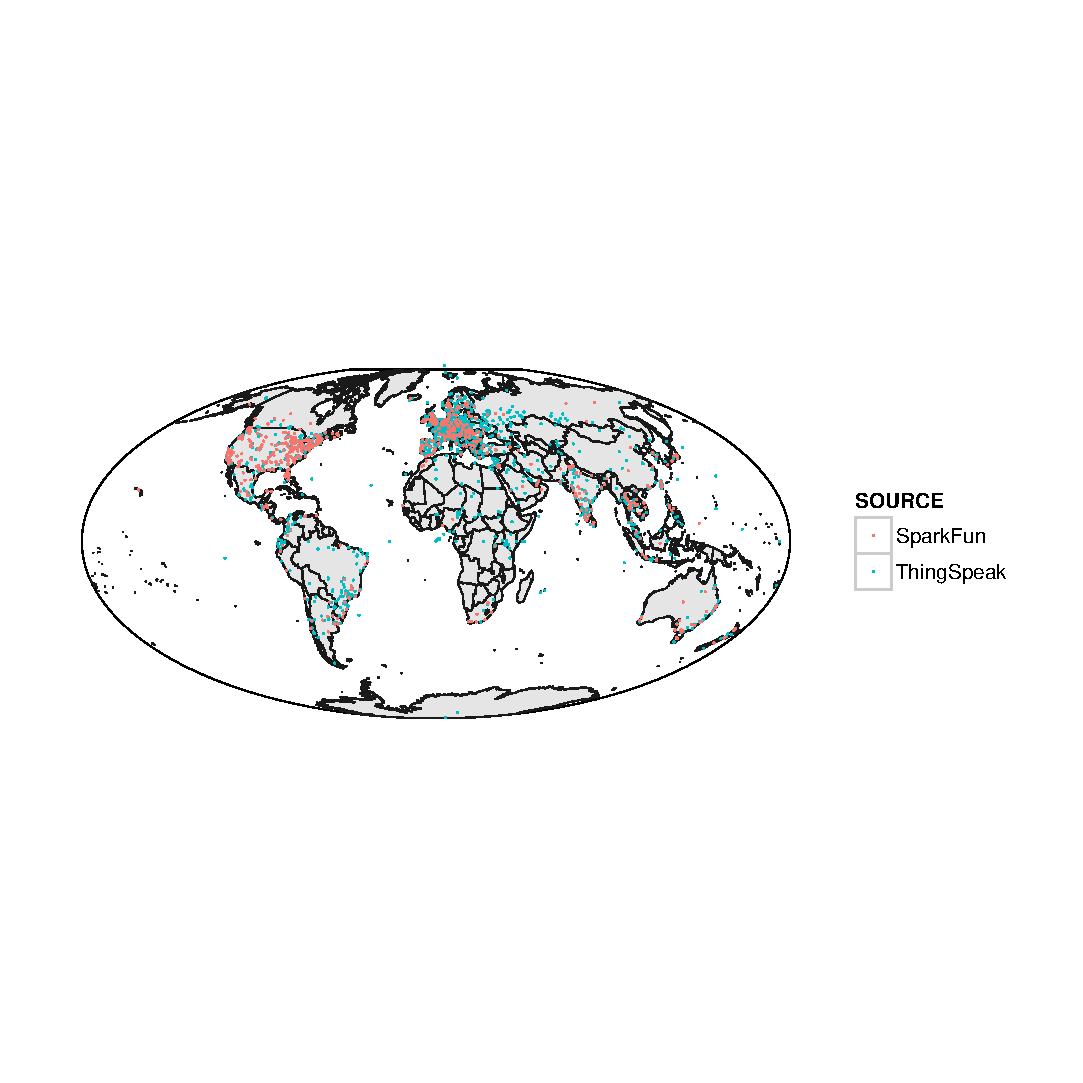
\includegraphics[width=1\textwidth]{img/map.eps} 
\caption{Location of all ThingSpeak and SparkFun sensing sources.}
\label{geo}
\end{figure*}

Given such results, the importance of information fusion from different sources is clear, since not only the sampling number of the sensing infrastructure is incremented, but also its coverage.
Indeed, ThingSpeak appears to have much more utilization in the European region, whereas SparkFun seems to be more popular in North America.
Furthermore, this consideration might be extended to different macro topic areas, meaning that some open data sources are specialized on a specific field of measuring.
For instance, governmental sources providing open data such as EPA (United States Environmental Protection Agency) \cite{epa} are primarily focused on environmental data, whilst crowdsensing sources such as OpenSignal \cite{opensignal} regard measurements on cellular network signal strength and coverage.
\\

Therefore, a basic unification counting on an essential set of metadata is crucial, composing the minimum skeleton to which a data stream should be linked.
For such purpose we aim to design an unique ID assignment policy, a geolocalization (with a precision error), a freshness of the information (given by the last update timestamp), a friendly name and an inferred measurement category (such as temperature, humidity and so on) together with an unit of measure.

%[TODO FEEDBACK]